\documentclass[11pt,a4paper,oneside]{report}
%\usepackage[utf8]{inputenc}
\usepackage[a4paper,width=150mm,top=25mm,bottom=25mm]{geometry}
\usepackage{listing}
\usepackage{enumerate}
\usepackage[fleqn]{amsmath}%mathtools includes this so this is optional
\usepackage{natbib}
\usepackage{amssymb, amsthm}
\usepackage{float}
\usepackage{ bbold }
\usepackage{amsfonts}
\usepackage{amssymb}
\usepackage{graphicx}
\graphicspath{{image/}}
\usepackage{times}
\usepackage{nomencl}
\usepackage{amsmath}
\usepackage{appendix}
\usepackage{setspace}
\usepackage{color}
\usepackage{fancybox}
\usepackage{lipsum}
\usepackage{relsize}
\usepackage{environ}	
\usepackage{fancyhdr}
\pagestyle{fancy}
\fancyhead{}
\fancyhead[RO,LE]{Risk Sensitive Markov Decision Process and Linear Programs}
\fancyfoot{}
\fancyfoot[LE,RO]{\thepage}
\fancyfoot[LO,CE]{Chapter \hspace{0.6mm}\thechapter}
%\fancyfoot[CO,RE]{Prakash}
\renewcommand{\headrulewidth}{0.4pt}
\renewcommand{\footrulewidth}{0.4pt}

%\usepackage[bookmarks=true]{hyperref}
%\usepackage{caption}
%\usepackage{subcaption}
%\usepackage[utf8]{inputenc}
%\usepackage{amsmath}
%\usepackage{amsfonts}
%\usepackage{amssymb}
%\usepackage{graphicx}
\date{}


%\fancyhf{}

%\fancyhead[RE]{\it{\nowuppercase{\leftmark}}}
%\fancyhead[LO]{\it{\nowuppercase{\rightmark}}}
%\fancyfoot[CE,CO]

\begin{document}
\begin{titlepage}
\begin{center}
%\vfill
	\vspace*{1cm}
	\Large
	A Report\\
	\vspace{0.5cm}
	\Large
	on\\
	\vspace{0.5cm}
	\Huge
	\textbf{"Finite Horizon Markov Decision Programs and Linear Programs"}\\
	\vspace{0.5cm}
	\vspace{1.5cm}
	\Large
	\textbf{Submitted in partial fulfillment of the requirements}\\
	\vspace{0.5cm}
	\Large
	of  the degree of\\
	\vspace{0.5cm}
	\Large
	\textbf{Master of Technology}\\
	\vspace{0.5cm}
	\Large
	by\\
	\vspace{0.2cm}
	\Large
	\textbf{(Gawas Prakash Arjun)}\\
	
	%\vspace{0.5cm}
	\Large
	(Roll no. 153190008)\\
	\vspace{0.5cm}
	\Large
	Supervised by\\
	\vspace{0.2cm}
	\Large
	\textbf{(Prof. Veeraruna Kavitha)}\\
	\textbf{(Prof. Ashutosh Mahajan)}\\
	\vspace{0.8cm}
	{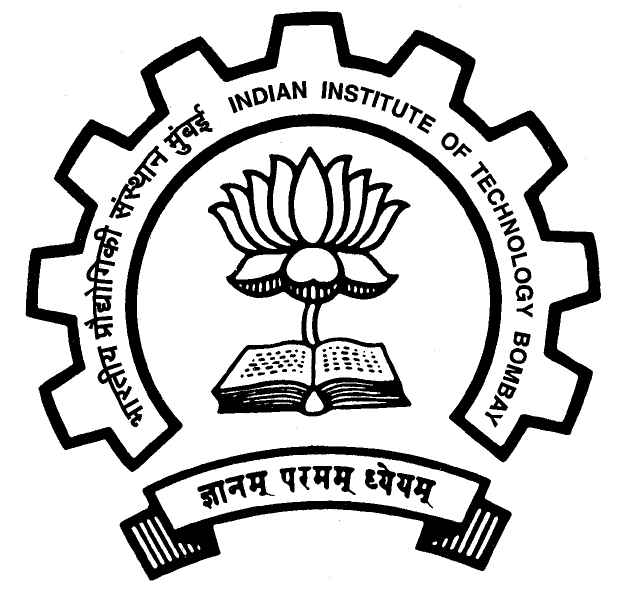
\includegraphics[scale=0.1]{logo.jpg}}\\
	\Large
	Inter-disciplinary program\\
	\Large
	in\\
	\Large
	Industrial Engineering and Operations Reserach (IEOR)\\
	\Large
	IIT BOMBAY\\
	\Large
		(2016-17)
\end{center}
\end{titlepage}
%\chapter*{Approval sheet}
%This is to certify that 
\chapter*{Declaration}
I declare that this written submission represents my idea in my own words and where others's idea or words have been included ,I have adequately cited and referenced the original source.I also declare that I have adhered to all principles of academic honesty and integrity and have not misrepresented or fabricated or falsified any/data/fact/source in my submission.I understand that any violation of the above will be cause for disciplinary action by the institute and can also evoke penal action from the sources which have thus not been properly cited or from whom proper permission has not been taken when needed.
\vspace{1cm}


\noindent Date:\hfill Prakash Arjun Gawas                     
\begin{flushright}(153190002)\end{flushright}
\chapter*{Acknowledment}
I would like to extend thanks to the many people who so generously contributed to the work presented in the thesis.Special mention goes to my enthusiastic supervisors, \textbf{Prof. Veeraruna Kavitha} and \textbf{Prof. Ashutosh Mahajan} for giving me opportunity of working under their guidance. Their direction, motivation, affectionate guidance and support have been the source of inspiration to bring the report this shape. I thank all the other faculty member of Industrial Engineering And Operations Research, who made me realize the virtue of learning through sustained hard work.
\vspace{6mm}

\noindent I would like to thanks all those whose name I missed but have contributed in any form for building up of the thesis upto now.
\vspace{1cm}

\begin{flushright}
Prakash Arjun Gawas\\
(153190002)
\end{flushright}

\chapter*{Abstract}
The project is based on the Finite Horizon Markov Decision Problems with risk sensitive cost. Classical MDPs are based on optimizing the expected value of the total sum cost for all the periods (also called risk neutral cost), to find the optimal policies. This only considers the mean total cost and does not give any importance to fluctuations around the mean.DP and LP solution approaches are very  well  defined for linear MDPs. In risk sensitive cost we will give due importance to higher moments of this total cost by optimizing the expected value of the exponential value of sum cost. This is an example of multiplicative MDPs. Recently an LP based solution is provided for solving the finite horizon Risk MDPs using appropraite risk parameter. Using these LPs I intend to solve the classic case of Inventory Control problem. The optimal policies for the problem are very well known and are of the type (s,S): order quantity S-x, if stock x drops below s, so that the inventory level reaches S. These policies were shown to be optimal for linear ordering, shortage and holding costs. OUr main aim  was to study optimal policies for risk sensitive costs. The results of our study showed $(s,S)$ to be optimal for risk sensitive cost also. Also the convergence of risk sensitive policy to linear cost policy was confirmed as risk parameter approaches zero.
\tableofcontents
\listoftables
\chapter{Introduction}

Markov Decision process (MDP) is a mathematical framework that solves the problem of sequential decision making under uncertainty, to obtain an optimal policy. At each decision epoch the system state provides the decision maker with all necessary information for choosing an action from available actions in that state. As result of an action the decision maker receives an immediate reward and the system state evolves to a possibly different state at the next epoch depending on the controlled (action based) transition probability. Each action, the decision maker chooses in any particular state and at any time slot t, will have an associated reward/running cost $(R_t)$. The reward depends also on the current system state. In case of finite horizon problems, it also considers a terminal cost that only depends upon the state at termination. Hence over time the decision maker will receive a sequence of reward/costs.\\

\noindent A policy is a sequence of such actions/rules, which the decision maker chooses at any time epoch depending on the state of the system. The aim of MDP is to find a policy prior to the first decision epoch that maximizes the expected value of a function $f$ of the reward sequences. In general MDP optimizes the expected value of the function $f$ that defines a way of aggregating the running costs related to all the time slots under consideration, i.e., to optimize $E[f(R_1,R_2,...)]$. Linear MDPs consider expected value of either sum of all the running costs $E[\sum_t{R_t} ]$, or sum of discounted values of all the running costs $E[\sum_t{\beta^t {R_t}} ]$ with discount factor $\beta<1$, or time average of the running costs $\lim_{T \to \infty}{[E[ \sum_{t\leq T}{R_t}]}{/T}$ .They are respectively called total cost, discounted cost or average cost problems. Also MDP whether discounted or total cost, can either be modelled over a finite time horizon or over the infinite time horizon. \\


\noindent Linear MDPs, also called risk neutral MDPs, control the first moment (expected value) of the sum cost. Optimization of the expected cost of an MDP is well studied. Many approaches have been developed to solve the problem. Dynamic programming (DP) is very popular technique to find optimal policies for finite horizon problems. Dynamic programming involves finding the optimal expected cost using Backward Induction. It basically solves a big problem by dividing it into many sub problems and than optimizing these sub problems. The corresponding equations are called optimality equations \citep{puterman1990market}. This gives rise to what is known as the Principle of Optimality where no matter what the current state and initial decision are, the remaining decisions must constitute an optimal policy with regard to the state resulting from the first decision. Others solution methods include Value Iterations, Policy iteration and their variants. These are iterative algorithms based on fixed point equations derived from the Optimality equations and the theory of contraction mappings on normed linear spaces. The relationship between discounted MDPs and Linear programs (LPs) is also pretty well defined. Though not efficient, LPs have elegant theory: ease in addition of additional constraints and facility of sensitivity analysis make it very attractable in some cases. LPs are derived based on properties of the solutions to the optimality equations (see Theoram 6.2.2, \cite{puterman1990market}). Primal linear program finds the optimal value while its dual provides the optimal policy.\\


In some situations we may also want to control the fluctuations around the expected value, which calls for Risk Sensitive MDPs (RSMDPs). RSMDPs can have varied applications in diverse fields. From investment of funds to manufacturing processes one can use RSMDPs to find optimal decisions. RSMDPs basically mean giving varied importance to higher moments of the total expected cost. One can also just optimize a function of mean and variance only as in \citep{mannor2011mean}.  The literature on RSMDPs is relatively limited though. In \cite{howard1972risk}, Howard and Matheson have considered the maximisation of total reward with a constant risk sensitive parameter. They have discussed the application of iterative algorithms like Value Iteration and Policy Iteration to risk sensitive case. Recently in [\citep{kumar2015finite}] ,authors have proposed an LP based approach to solve the RSMDPs for finite horizon problem. Also they have augmented the state space appropriately so as to make addition of more constrains simple to solve the constrained RSMDP. The relation between LPs and infinite horizon is even more complex and needs to be investigated.\\ 


\noindent MDPs can be applied to varied examples in real life situations. One such application is the classic inventory control problem. In INVENTORY CONTROL problem the decision maker must decide how much to order in each time period to meet demand for its products. The demand  is considered to be stochastic, whose distribution function is known. The objective here is to find a policy of ordering at any time epoch so as to minimize the total cost incurred for total period of time $T$ thus making it a finite horizon problem. The various cost incurred depends on the current state of inventory, amount ordered and demand in that time period. There are three basic costs considered in this situation. Ordering cost that includes total  ordering cost of the quantity and also fixed order set-up cost. Holding cost for storing inventory and carrying it into the next period. Shortage cost is applicable when we cannot fulfil the demand on hand. All the costs are considered to be linear. Hence given the state and the amount to be ordered in the current period the next inventory level will only depend on the demand in the current state and will transition according to the demand distribution.  First we model it into a sequential decision model defining appropriate state space, actions, transition probability and rewards at each time epoch.  If we solve this problem using one of the techniques mentioned previously, the policy that the decision maker has to follow to optimize the expected reward only  is of the type (s,S).In \cite{scarf1959optimality}, Herbert Scarf has shown that when holding cost and shortage cost are linear then the optimal policy is of this type. This means that whenever the inventory level goes below the level s will order so as to increase are inventory level to S, if not than we will not order.  The aim in my work is to find optimal policies for a risk averse decision maker. Authors in \citep{kumar2015finite} has given LP model for risk sensitive MDPS which can be applied for this example. \\

In Chapter III the model for inventory control is defined with the used notations. The rewards pertaining to the linear MDP have been identified. There were two ways in which we could model the rewards for this problem. One way was that given the current state of the inventory and the action we can find the average reward at that point. Other was to shift the holding and shortage cost from the current period to the next period. Both the cases were solved using LP formulation given in \citep{kumar2015finite} for optimising the linear expected cost and also by using dynamic program from \citep{puterman1990market} and the results were validated. Furthermore in Chapter V the model for risk sensitive MDPs is presented.

\chapter{Literature Survey}


\noindent Classical MDPs deal with the maximisation of cumulative reward, however a decision maker may focus on several other distributional properties. Most decision makers may be risk averse i.e. they would like to reduce their risk and thus this forms the basis of a risk sensitive model. 
One way is to focus on mean and variance of the cumulative reward. Mean-variance optimisation has varied applications from finance to manufacturing fields.\\

\section{Mean Variance Optimization}
In \cite{mannor2011mean}, authors consider mean variance optimization, that is they consider optimizing 
\begin{equation}
E[\sum_t R_t] - \theta Var(\sum_t R_t)
\end{equation}
With the introduction of variance in the cost function, we can optimize the fluctuations around the mean. They also deal with various computational complexities of mean-variance optimisation. There many problems associated with Mean-Variance MDPs.
\begin{enumerate}
\item The main problem with mean-variance optimisation is the absence of principle of optimality which could have led to simple recursive algorithms. For example consider a situation where the decision maker has received unexpected high rewards in the initial stages and has got to a state. He than may incur losses to keep the variance small. In case the user is at the same state and at the same stage, however received low rewards before this stage, then it would receive higher rewards in the later stages. Thus the principle of optimality fails. 
\item Also variance $ (Var(W))=E(W^2)- (E(W))^2$ is not a linear function of the probability measure of the process where $W$ is sum of the rewards for the time horizon.
\item These MDPs are typically NP hard but may admit a pseudo polynomial time solution.
\end{enumerate} 
They have defined their MDP model and compared different types of policies classes. Given the MDP model $M$ (defined by the time horizon, state space, set of actions, set of rewards, transition probability) and rational numbers $\lambda$, $\nu$ the question they are addressing is whether there exist a policy in the set  ${\prod}$ such that $J=E(W)\geq \lambda$ and $V=Var(W)\leq \nu$. They  and established NP-hardness of this problem for all type of policies. They have addressed this using constrained Markov Decision Process to develop pseudo polynomial exact or approximate algorithms.
To develop exact algorithms they augment the state space , to include the a term that contains the sum reward until the given stage. Considering bounded integer rewards, they have identified cases for the existence of exact pseudo polynomial time algorithms.  LP approach cannot be used directly used for the problem due to convexity issues in Mean Variance MDPs. Hence they have concentrated on the pair $J$ and $Q = E[W^2]$ and for integer rewards established the existence of pseudo polynomial solution.
In developing approximate algorithms the authors precisely consider the following:
\begin{itemize}
\item Minimize V while J $\geq \lambda$
\item Maximize J while V $\leq \nu$
\end{itemize}
On similar lines as previously they consider integer rewards the authors have proved existence of a polynomial time algorithm. For any general reward case we can discretize the rewards and obtain new MDP which will be equivalent to one with integer rewards and the same algorithm can be applied.\\

In \citep{filar1989variance}, Filar et al has given a Quadratic Program (QP) to directly solve Mean-Variance MDP ($_{**}$). The constraints of the QP are similar to the usual LP constraints, but the objective is quadratic in nature \cite[equations(2.9)]{filar1989variance}. This is convex constrained QP.
In \cite{gosavi2006risk},the author again considers the Mean-Variance problem($_**$) to design plans for total productive maintenance (TPM). TPM  focuses on improving the overall effectiveness of a manufacturing facility by eliminating the waste of time and resources. Their aim was to find optimal productive maintenance (PM) time. PM help reduce the frequency of unexpected repairs when failure rate is of increasing nature. Traditional approaches in TPM only used expected value of the long run cost and overlooked the risk associated with the high cost. In actual practice risk sensitive managers would use the expected value of long-run cost and then use a factor of safety for the same optimal time. This is a heuristic approach and is more conservative. They give mean variance model where the objective function is $g(\tau)= \mu_C+ \theta {\sigma}^2$ with $\theta>0$, where $\mu_C$ and $\sigma^2$ denote the long-run mean and the long-run variance, respectively, of the net cost per unit time incurred from following a preventive maintenance plan that prescribes $\tau$ as the time for PM.An alternative formulation in terms of rewards, in which the objective function is maximized,is $g(\tau)= \mu_R- \theta {\sigma}^2$ with $\theta>0$, where $\mu_R$ and $\sigma^2$ denote the long-run mean and variance of the net reward per unit time, respectively. Risk neutral models have $\theta =0$. Typically $\theta$ is selected experimentally. TPM plans for the production line in its entirety tend to be distinct from those for individual units that operate independently of the line. Hence they have developed separate models for the individual-unit scenario and the production-line scenario. For the case of the individual unit, a renewal-theory model is used. He considers a sub-optimal problem by considering the optimal among the age replacement policies. A typical age replacement policy replaces the item when its age reaches $\tau$ or when the failure occurs. Therefore the MDP crumble downs to a single variable optimization problem. Here every failure or a maintenance triggers a so-called renewal event. Using Renewal Reward Theory he has derived an expression for $g(\tau)$ in terms of $\tau$, failure distribution and the individual cost of repair and maintenance. For the case of the production line a more involved model based on MDPs is used. He first develops the MDP identifies a Quadratic Program given in [] to solve the MDP. But solving the QP this is computationally expensive. He present an approach based on linearising the quadratic objective function by using a surrogate form for variance. Optimization could then be performed via linear programming. The existence of a deterministic policy is then proved for the surrogate objective function using DP approach to solve the problem by deriving the necessary optimality conditions. Using this he proposes a PI algorithm and shows its convergence. Computational results showed that the surrogate function did mimic the exact function reasonably well and also proves convergence in relatively short period of time.\\

\section{Variants of Risk Sensitive MDPs}
Mean Variance MDP reduces the variance trying to optimize the mean cost. However several other authors have considered many alternative ways of optimizing the fluctuations around the mean.
In \cite{liu2005risk}, authors talk about risk sensitive planning with one switch utility functions. One switch utility functions model a decision maker whose decision change with their wealth level. For example a decision maker with low wealth levels may be risk averse, but may become risk neutral as the wealth level increases. These function model the risk attitude of decision maker.A decision maker is risk-neutral if their utility function is linear, risk-averse if their utility function is concave, and risk-seeking if their utility function is convex. Here one need to maximise the expected utility of a MDP for a given one switch utility function. This is difficult since the resulting planning problem is not decomposable. They model a probabilistic planning problem as a fully observable Goal-Directed Markov Decision Problems (GDMDPs) and investigate how to maximize the expected utility. The optimal course of action now depends not only on the current state of the GDMDP but also the wealth level. Thus the authors first gives an approach to transform the risk sensitive GDMDP (RS-GDMDP) into a risk neutral one by augmenting the state space of the RS-GDMDP with possible wealth levels. The authors than relate the values and policies of the original and augmented GDMDP.  The resulting RS-GDMDP has an infinite state space but its properties allow us to generalize the standard risk sensitive version of Value Iteration (VI) which manipulates to a risk sensitive version of VI, which manipulates the functions that map wealth level to values.\\

\section{Exponential form of Risk Sensitive MDPs}
As seen above Mean-Variance MDPs have several issues. However by considering exponential cost, one can also reduce the fluctuations around the mean. Exponential cost cover some of the drawbacks that are present in Mean-Variance MDPs.
In comparison with linear MDPs which control the first moment (expected value) of the sum cost, the risk sensitive MDPs also control the variability/fluctuations around the expected value, by considering the higher moments. In \cite{kumar2015finite}, the authors model finite horizon risk sensitive constrained MDPs using LP technique.  The aim is to give varying importance to sample path trajectories and the expected value, as controlled by a parameter $\gamma$. Depending upon $\gamma$, called the risk parameter, it provides importance to higher moments of the sum cost. The linear MDPs are viewed as risk neutral MDPs with $\gamma=0$. The aggregation function in this case equals the exponential of the sum of the running costs, $E[e^{-\gamma {\sum_{t\leq T}R_t}} ]$. Note that $E[e^{-\gamma {\sum_{t\leq T}R_t}} ]= E[{\sum_k \gamma ^k {(\sum_{t\leq T}{R_t}})^{k}}/{k!}]$, thus considering the higher moments of the sum cost.
The authors have considered the following transformation of the risk neutral objective function to capture the higher moments where $\alpha$ is the initial distribution and $\pi$ represents the policy .
\begin{equation}
\tilde{J_o(\alpha,\pi)} = (1/\gamma)\log(J_o(\alpha,\pi))
\end{equation} 
where
\begin{equation}
J_o(\alpha,\pi) = E^{(\alpha,\pi)}[e^{\gamma \sum_t r_t(S_t,A_t)]} 
\end{equation}
This the risk sensitive objective function. For smaller values $\gamma$ the objective takes the form:
\begin{equation}
\tilde{J_o(\alpha,\pi)} \simeq E^{(\alpha,\pi)}[ \sum_t r_t(S_t,A_t)] + (\gamma /2)Var^{(\alpha,\pi)}[\sum_t r_t(S_t,A_t)] 
\end{equation} 
As one can see as $\gamma \rightarrow 0$ the objective function approaches risk neutral cost. The value function is defined as the optimal value of the above risk sensitive objective with initial condition $X_0\equiv x$:
\begin{equation}
v^*(x):=min_{\pi\in\cal{D}}\tilde{J_o(\alpha,\pi)}  \text{for any } x\in \cal{X}
\end{equation}
The authors have given a Dynamic Programming equations using backward induction as below for any $x\in \cal{X}$.
\begin{align}
\begin{split}
v_T(x) &= r_T(x), \text{   and for any  } 0\leq t\leq T-1, \\ 
v_t(x) &=\min_{a\in \cal{A}}\bigg \lbrace r_t(x,a) + \frac{1}{\gamma}log\Big[\sum_{x'\in \cal{X}} p(x'|x,a)e^{\gamma v_{t+1}}(x')\Big]\bigg\rbrace, 
\end{split}
\label{eqn:1}
\end{align}
and their solution provides the value function $v*(x) = v_0^*(x)$. To simplify the above set equations, the following translation of the value function is used:
\begin{equation}
u_t(x) = e^{\gamma v_t(x)} \text{   for all } 0\leq t\leq T, \text{ and } x\in \cal{X}
\end{equation}
By monotonicity and continuity $u_0^*(x) = e^{\gamma v_0^*(x)}$ is the minimum value of the risk cost $J_0$ in equation[]:
\begin{equation}
u_0^*(x)=\min_\pi J_0(x,\pi).
\end{equation}
Hence the DP equations are now rewritten as:
\begin{align}
\begin{split}
u_T(x) &= e^{\gamma v_T(x)}, \text{   and for any  } \text{ for any } x\in \cal{X} \text{ and},\\
u_t(x) &=\min_{a\in \cal{A}}\bigg \lbrace e^{\gamma v_t(x)}\sum_{x'\in \cal{X}} p(x'|x,a)u_{t+1}(x')\bigg\rbrace, 
\end{split}
\label{eqn:1}
\end{align}
The solution of the above equations provide the translated value function vector $u^* = \lbrace u_t^*(t); 0\leq t\leq T-1, x\in \cal{X}\rbrace$. The authors than provide connection between DP equations and two appropriate LPs for finite horizon case. The primal LP (2) provides the value function while the dual LP provides the optimal policy. For LPs in risk sensitive MDPs the authors have circumvented this problem by incorporating the multiplicative cost term into the mapping that converts any given Markov policy to a feasible point of the LP. This due to the fact that it is possible to construct the linear objective function of the relevant LP using the running costs of all time slots but the cost accumulates in a multiplicative manner for risk sensitive MDPs and hence the same approach cannot be adapted directly for constructing an LP for risk MDP. Primal and dual LPs for finite horizon RSMDP are efficiently designed.  By substituting $\gamma=0$ in the Primal and Dual LP we get back to a risk neutral MDP which will maximise the expected cost. However there is inconsistency between those LP and they do not point to same optimal policies. They have identified this disparity between the LPs and have corrected the inconsistency.

\begin{equation}
\hspace{1cm}\text{max    }   \hspace{0.2cm}\sum\limits_{x\in\cal{X}}\alpha(x)u_0(x)
\end{equation}
\begin{equation*}
\begin{array}{ll@{}ll}
\text{subject to}& \\
&u_{T-1}(x)&\leq b_{x,a}                                                             &\text{ for all } x,a,\\
&u_t(x)&\leq e^{\gamma v_t(x)}\sum\limits_{x'\in \cal{X}} p(x'|x,a)u_{t+1}(x')   &\text{ for all } x,a \text{ and } t\leq T-2
\end{array}
\end{equation*}
$\hspace{0.9cm}\text{ with } b_{(x,a)}:= e^{\gamma r_{T-1}(s,a)}\sum_{s'} p(s'|s,a)e^{r_T(s')}.$\\
However when we need to add extra constraints to this model, the fact that costs are multiplicative poses a problem. The authors have proposed a technique to add more constraints to the LP by augmenting the state space with an extra component, which is representative of this multiplicative cost. The addition of this extra component makes it easy to add new constraints .They have also discussed two applications of the problem. First application includes delay tolerant networks where a message has to be transferred from a source to a faraway destination with the help of occasional contacts between the freely moving nodes (that are willing to become the relays) and the source/destination. Second application includes a lossy (finite buffer) queuing system with two server modes and with a constraint on the utilization of fast server mode. They have also compared the risk neutral policies with risk sensitive policies for the constrained MDP problem.\\

\section{Inventory Control}
In \cite{scarf1959optimality}, Herbert Scarf considers a dynamic inventory problem where he considers ordering costs, holding costs and shortage costs. The underlying assumption here is that the holding and shortage cost are linear. He shows that when this is true the optimal policy in each period is always of the type (S,s). This means that whenever the inventory level goes below level s will order so as to increase are inventory level to S, if not than we will not order. He builds a total cost function, composed of the three costs described above. This function can be used to construct a dynamic program equation. He shoes the total cost function follows K-convexity. Due to this the optimal policy the optimal policy turns out to be of such simple form.\\

\chapter{Inventory Control - Linear And Risk Sensitive MDP Framework}
\section{Inventory Control}
Inventory refers to idle goods or materials that are held by an firm for use sometime in the future. Items stored in inventory can vary from raw materials, purchased parts, finished goods etc. One reason firms maintain inventory is that it is rarely possible to predict sales levels, production times, demand, and usage needs exactly. Thus, inventory serves as a buffer against uncertain and fluctuating usage and keeps a supply of items available in case the items are needed by the firm or its customers. While inventory serves an important and essential role, the expense associated with financing and maintaining inventories is a substantial part of the cost of doing business. In large organizations, the cost associated with inventory can run into the millions of dollars.
Two important questions that must be answered in order to effectively manage inventories are as follows:
\begin{enumerate}
\item When should the inventory be replenished? 
\item How much should be ordered when the inventory is replenished?
\end{enumerate}

Sequential decision models have been widely applied to inventory control problems and are one its earliest applications. These models can be applied not only to find reorder points of single product, but also to complex multi product supply network. In this work, I consider a single product Inventory control system and try to find optimal reorder points. Under various scenarios it is proved that $\mathcal{(S,s)}$ policy is optimal (e.g., \citep{scarf1959optimality}) when one considers optimizing the expected value of the costs in Inventory control. As a first part of my work, using numerical methods i.e dynamic programming and LPs I proved the optimality of $\mathcal{(S,s)}$ in one example scenario.I have also considered risk sensitive cost (expected value of exponent of total costs) and studied the differences in the two optimal policies.

\section{Model}
Consider an Inventory storage that can be stocked with goods to a maximum size of $M$. Results proving optimality of (S,s) policy (e.g., \citep{scarf1959optimality}) often do not consider a limit on inventory size, however due to limitation of numerical computations we assume $M$ as the maximum inventory size possible.  This is also a realistic scenario. Let $N$ be the number of planning horizons. A sequence of ordering decisions is made at the beginning of number of equally spaced intervals. The inventory builds upon ordering stock and depletes on fulfilling demand. Following assumptions apply to the model 
\begin{enumerate}
\item[\textbf{1)}] Demand $\xi_1, \xi_2.....\xi_N$ are independent and identically distributed by a common discrete distribution function $P(\xi)$.
\item[\textbf{2)}] All orders are placed at the start of the period and received immediately and lag is zero.
\item[\textbf{3)}] Demands arrive immediately after the orders arrive and are fulfilled instantly.
\item[\textbf{4)}] Holding and shortage costs are charged linearly.
\item[\textbf{5)}] Unsatisfied demand is lost forever.
\end{enumerate}
\noindent Now to define the different costs associated with the inventory process.
\begin{enumerate}
\item[\textbf{1)}] Order cost $(C_O)$ : This contains two components:
\begin{enumerate}
\item[\textbf{a)}] Fixed order cost (K) : This the fixed cost for an order irrespective of the number of units ordered.
\item[\textbf{b)}] Variable cost : This is a linear cost cost directly proportional to number of units ordered.Thus the order cost when quantity $a$  is ordered equals:\\
\end{enumerate}
\begin{equation}
C_O(a) = 
\begin{cases}
0 ,            &a=0\\
K+ c_u, {a} ,                &a>0
\end{cases}
\end{equation}

\hspace{6mm} where  $c_u$  is the unit price.

\item[\textbf{2)}]Holding cost $(C_H)$ : Cost associated with storing the inventory that remains unsold. This cost will depend on the demand.

\begin{equation}
C_H(s,a) = 
\begin{cases}
0,   &\xi \geq s+a\\
c_H(s+a-\xi),     & \xi <s+a
\end{cases}
\end{equation}
\begin{flushleft}where $c_k$ is the unit holding cost.
\end{flushleft}

\item[\textbf{3)}]	Shortage cost$(C_S)$ : Cost associated with not being able to fulfil demand from the stock. 

\begin{equation}
C_S(s,a) = 
\begin{cases}
0          &,\xi \leq s+a\\
c_S(\xi-s-a)     &  ,\xi >s+a
\end{cases}
\end{equation}
\begin{flushleft}where $c_s$ is the unit shortage cost.
\end{flushleft}
\end{enumerate}
Hence now the total expected cost to be charged for any period $t$will be:
\begin{equation}
= (K+ c_u {a})\mathbf{1}_{\lbrace a>0\rbrace} + \sum_{\xi=0}^{s+a-1}c_H(s+a-\xi)P(\xi) + \sum_{\xi=s+a}^{\infty}c_S(\xi-s-a)P(\xi)
\end{equation} 
We now describe a sequential model to determine the optimal reorder points for single product inventory system. Decision epoch will be the review of the inventory level after each interval. The system state is the inventory level at the time of review. In a given state the action correspond to the amount of stock the order is placed for. Note that in our case we maximum order quantity so that are total inventory would not be greater than $M$. Once the order has been placed for a given state, the transition probabilities will depend on the quantity ordered and the random customer demand for the product in the period. After the demand is fulfilled we incur a cost (ordering + shortage + holding) depending on the order, stock on hand and the random demand. A decision rule will provide us the quantity to be ordered, given the state of the inventory at the time of review. Thus we seek a policy that consists of such decision rules to minimize the total cost of the entire planning period. 
A Markov decision process formulation follows below:\\

\noindent Decision Epochs:\\
\begin{equation*}T = \lbrace 1,2,3,...N \rbrace,\hspace{1.5cm}   N \leq \infty. 
\end{equation*}\\
\noindent State space:\\
\begin{equation*}S = \lbrace 0,1,2,...M \rbrace  
\end{equation*}\\
\noindent Actions:\\
\begin{equation*}A_s  = \lbrace0,1,2,...M-s \rbrace
\end{equation*}\\
where $s\in S$\\
\noindent Expected Rewards:\\
\begin{equation*}r_t(s,a) = (C_O(a) + C_H(s,a) + C_S(s,a)) 
\end{equation*}\\
\noindent Terminal reward $r_T(s)=0$.
\noindent \\Transition Probability:\\
\begin{equation*}
p(j|s,a)=
\begin{cases}
P(\xi= s+a-j),&{s+a}>j\geq0\\
P(\xi\geq s+a),&j=0\\
0,&\text{else}
\end{cases}
\end{equation*}
\section{Linear Cost - Standard MDP Model}
\subsection{MDP with cost considered in the same period}
Our objective is to minimize the expected value of the sum of all running costs, that is $E[\sum_t r_t(s,a) ]$.
This equivalent to optimizing:
\begin{align}
E[\sum_t r_t(s,a) ]&=\sum_t E[r_t(s,a)] \\
&= \sum_t E \bigg[ E\Big[{R_t}|{(S_1,A_1),(S_2,A_2),...,(S_{T-1},A_{T-1}),(S_T)}\Big]\bigg].
\end{align}
\noindent Hence given the current state $s$ and action to be taken $a$ we can find the cost any period $t$. The  cost $r_t$ for the period $t$ will depend only on the state $s_t$ and the action$a_t$ in that period and can be calculated as follows:
\begin{align}
\nonumber
E[R_t(s,a)|{(S_t=s,A_t=a)}] &=  E[C_O(a) + C_H(s,a) + C_S(s,a)]\\
\end{align}
This quantity is easy to compute, given $s$, $a$ and the distribution of demand $\xi$.
Hence now we can compute $E[r_t(s,a)]$ by simply multiplying with the probabilities $\lbrace P( S_t=s, A_t=a)\rbrace$

In \citep{kumar2015finite}, authors have given a Primal and Dual LPs to solve finite horizon linear program. The primal will give us the optimum cost, while the dual gives the optimum policies. The dual LP is given below.\\
\begin{align}
min\hspace{0.5cm} \sum_{t=1}^{T-1} \sum_{a_t} \sum_{s_t} r_t(s_t,a_t)y(t,s_t,a_t) + \sum_{a} \sum_{s,s'}r_T(s')y(T-1,s,a)p(s'|s,a)
\end{align}
\begin{flushleft}
\text{subject to:}
\end{flushleft}
\begin{align*}
&\sum_a y(0,s',a)=\alpha(s')     &\text{for all } s'\in S \\
&\sum_a y(t,s',a)=\sum_a \sum_s p(s'|s,a)y(t-1,s,a)    &\text{for all } 1\leq t\leq T-1 \text{ and } s'\in S   \\ 
&\text{and } y(t,s,a)\geq 0 \text{ for } a\in A_s \text{ and } s\in S. 
\end{align*}


Using the above LP we solve the inventory problem and results are given in chapter 5. The Above MDP model is  applicable for any discrete distribution of demand. But if the demand was to be continuous than we would need to change the MDP model as state space becomes infinite in that case and we need to come up with a idea. Then we would need to discretize the demand to keep the state space finite. 
\subsection{MDP after shiting the cost terms}
There is another way which can be used to represent the rewards in this MDP model. We consider  shift of few cost terms (from any time slot to its next), which would not change the actual problem and which would pave way for risk MDP. In formulation given in eq [], the holding and shortage costs depend upon the current inventory, order quantity and demand. In actual it depends only on the next state. It is easily known that if the state $s$ at the start of next period is greater than zero than we would directly incur holding cost equivalent to $c_hs$ in the current period. Therefore we can model the cost $r_t$ as function of the next state of inventory which would give us information on which of the cost is applicable in the previous period. So one can shift the holding and shortage costs to the next period where we would know the state. If $s=0$ than we for sure know that there was no holding cost and only shortage cost would apply.
Hence in this case we need to model the excess demand, when the state is zero. The reason for modelling the rewards this way is highlighted in the next section where we model Risk Sensitive MDPs. Considering this we can use the following:\\
\begin{equation}
r_t(s_t,a_t)=
\begin{cases}
c_{o}a_t&,t=1\\
c_{o}a + c_h(s_t)\mathbf{1}_{\lbrace s_t>0\rbrace} + c_s(\tilde{\xi})\mathbf{1}_{\lbrace s_t=0\rbrace}&,1<t< T\\
c_h(s_t)\mathbf{1}_{\lbrace s_t>0\rbrace} + c_s(\tilde{\xi})&,t=T
\end{cases}
\end{equation}
\noindent where $\tilde{\xi}$ is the excess variable demand and distribution of whose is to be known to compute the reward. This excess demand $\tilde{\xi}$ depends on the inventory state, the action taken in that state and demand in that period. Note that there exist terminal reward in this case. Hence with these new rewards, we can again solve the LP to get the optimal policy. Section 4.2 provides the results for this way of modelling. 
Advantages of this formulation:
\begin{enumerate}
\item The holding cost does not depend on random demand.
\item Shortage cost depends only upon excess demand $\tilde\xi$, which would than be independent of further state evolution. Further if the demands are memoryless, than $\tilde{\xi}$ has the same distribution as $\xi$.
\end{enumerate}

\section{Risk Sensitive MDP}
In risk sensitive MDPs we want to give importance to higher moments of the total rewards. Hence our objective is to optimize $E[e^{\sum_{t=1}^T \gamma r_t}]$
\begin{align}
E[e^{\sum_{t=1}^T \gamma r_t}]&=E[\Pi_{t=1}^Te^{ \gamma r_t}]\\
\nonumber
&=E \bigg{[}E\Big[\Pi_{t=1}^{T}e^{\gamma R_t}|(X_1,X_2,...X_T)(A_1,A_1,...A_{T-1})\Big]\bigg] 
\end{align}
\\ As compared to linear cost MDPs we cannot simplify this easily. If one notices in linear MDPs \ref{3.2}, we can simplify the total in terms of sum of expectations of the costs which is easy to compute as in \ref{3.1} .But this is not the case in Risk sensitive MDPs as seen above and we cannot average out the risk reward for a given state $s$ and the corresponding action $a$.  Hence using we need to use the technique where we shift the rewards to the next time period. We will consider a the transformed risk reward as below:
$E[e^{\sum_{t=1}^T \gamma r_t}]$
\begin{align}
&=E \bigg{[}E\Big[\Pi_{t=1}^{T}e^{\gamma R_t}|{(X_1,A_1),(X_2,A_2),...,(X_{T-1},A_{T-1}),(X_T)}\Big]\bigg]
\end{align}
substitute the shifted reward from equation
\begin{align}
&=E[E[\Pi_{t=1}^{T-1} e^{c_o A_t}\Pi_{t=1}^{T}e^{(c_h S_t)\mathbf{1}_{\lbrace S_t>0\rbrace}+(c_s \tilde{\xi})\mathbf{1}_{\lbrace S_t=0\rbrace}}|(X_1,X_2,...X_T)(A_1,A_2,...A_{T-1})]]\\
\nonumber
&=E[\Pi_{t=1}^{T-1} e^{c_o A_t}\Pi_{t=1}^{T}e^{(c_h S_t)\mathbf{1}_{\lbrace S_t>0\rbrace}}E[\Pi_{t=1}^{T-1}e^{(c_s \tilde{\xi})\mathbf{1}_{\lbrace S_t=0\rbrace}}|(X_1,X_2,...X_T)(A_1,A_2,...A_{T-1})]]
\end{align}
In the above rewards the shortage cost depends on the random quantity $\tilde\xi$ (excess demand). The distribution of excess demand $\tilde\xi$ in general depends upon the inventory state and action of previous slot, however will not influence further evolution of the system.  We can assume memory less demands (geometric), in which case $\tilde\xi$ is again distributed geometrically and one can average this out to compute the shortage cost.
\begin{align}
E[\Pi_{t=2}^{T}e^{(c_s \tilde{\xi})\mathbf{1}_{\lbrace S_t=0\rbrace}}|(X_1,X_2,...X_T)(A_1,A_2,...A_{T-1})]&=E[\Pi_{t=1}^{T-1}e^{(c_s \tilde{\xi})\mathbf{1}_{\lbrace S_t=0\rbrace}}]\\ \nonumber
&=\Pi_{t=2}^{T}E[e^{(c_s \tilde{\xi})\mathbf{1}_{\lbrace S_t=0\rbrace}}]
\end{align}
Hence now we can write the transformed formed of the rewards as below:
\begin{equation}
r_t(s_t,a_t)=
\begin{cases}
c_{o}a_t&,t=1\\
c_{o}a + c_h(s_t)\mathbf{1}_{\lbrace s_t>0\rbrace} + \tilde{c})\mathbf{1}_{\lbrace s_t=0\rbrace}&,1<t< T\\
c_h(s_t)\mathbf{1}_{\lbrace s_t>0\rbrace} +\tilde{c}\mathbf{1}_{\lbrace s_t=0\rbrace}&,t=T
\end{cases}
\end{equation}
where $\tilde{c} = log(E[e^{(\gamma c_s \tilde{\xi})}]). $\\
Under this assumption one can apply directly use the risk sensitive LP (12)to solve the MDP model from \citep{kumar2015finite}. If we let $\gamma\rightarrow0$, authors in \citep{kumar2015finite} have shown that the risk sensitive cost converges to risk neutral cost. Similarly in this model the LP will converge to risk neutral LP. In the appendix the convergence of the risk sensitive cost is shown. This is an important step since $\tilde c$ is a function of gamma.
\pagebreak
\begin{align}
min\hspace{0.5cm} \sum_a &\sum_{s} b_{(x,a)}y(T-1,s,a)
\end{align}
\text{subject to:}
\begin{align*}
\sum_a y(0,s',a)&=\alpha(s')     &\text{ for all } s'\in S \\
\sum_a y(t,s',a)&= \sum_a \sum_s e^{\gamma r_{t-1}(s,a)}p(s'|s,a)y(t-1,s,a) &\text{for all } 1\leq t\leq T-1 \text{ and } s'\in S
\end{align*}
$
\text{ with } b_{(x,a)}:= e^{\gamma r_{T-1}(s,a)}\sum_{s'} p(s'|s,a)e^{r_T(s')} \text{ and } y(t,s,a)\geq 0 \text{ for } a\in A_s \text{ and } s\in S.$


\chapter{Results}
\section{Risk Neutral MDP}
\subsection{Uniform Demand Distribution}
Consider demand to be uniformly distributed with parameters ${\lbrace0,20\rbrace}$. Let $M = 20, N = 10, K = 0.5, c_u = 0.4, c_h=0.2, c_s=0.8$. Given these we can compute the rewards $r_t(s,a)$ by using [equation 3.2] and the necessary transition probability $p(s'|s,a)$ for the problem. These computations were carried out in MATLAB and the data was formatted appropriately to be given s input to the LP solver. The LP was modelled using AMPL. The results are shown in table \ref{t1} below. The table shows the optimum policy i.e. the optimum ordering quantity at any time stage at any inventory level.
\begin{table}[H]
\centering
\caption{Optimal Policy for Uniform Distribution with parameters $(0,20)$}
\label{t1}
\begin{tabular}{|c|c|c|c|c|c|c|c|c|c|c|c|}
\hline
\textbf{}        & \multicolumn{11}{c|}{\textbf{Decision Epoch}}                                                                                                 \\ \hline
\textbf{States↓} & \textbf{0} & \textbf{1} & \textbf{2} & \textbf{3} & \textbf{4} & \textbf{5} & \textbf{6} & \textbf{7} & \textbf{8} & \textbf{9} & \textbf{10} \\ \hline
\textbf{0}       & 14         & 14         & 14         & 14         & 14         & 14         & 14         & 14         & 13         & 8          & 0           \\ \hline
\textbf{1}       & 13         & 13         & 13         & 13         & 13         & 13         & 13         & 13         & 12         & 7          & 0           \\ \hline
\textbf{2}       & 12         & 12         & 12         & 12         & 12         & 12         & 12         & 12         & 11         & 6          & 0           \\ \hline
\textbf{3}       & 11         & 11         & 11         & 11         & 11         & 11         & 11         & 11         & 10         & 5          & 0           \\ \hline
\textbf{4}       & 10         & 10         & 10         & 10         & 10         & 10         & 10         & 10         & 9          & 0          & 0           \\ \hline
\textbf{5}       & 9          & 9          & 9          & 9          & 9          & 9          & 9          & 9          & 8          & 0          & 0           \\ \hline
\textbf{6}       & 8          & 8          & 8          & 8          & 8          & 8          & 8          & 8          & 7          & 0          & 0           \\ \hline
\textbf{7}       & 7          & 7          & 7          & 7          & 7          & 7          & 7          & 7          & 6          & 0          & 0           \\ \hline
\textbf{8}       & 6          & 6          & 6          & 6          & 6          & 6          & 6          & 6          & 0          & 0          & 0           \\ \hline
\textbf{9}       & 0          & 0          & 0          & 0          & 0          & 0          & 0          & 0          & 0          & 0          & 0           \\ \hline
\textbf{10}      & 0          & 0          & 0          & 0          & 0          & 0          & 0          & 0          & 0          & 0          & 0           \\ \hline
\textbf{11}      & 0          & 0          & 0          & 0          & 0          & 0          & 0          & 0          & 0          & 0          & 0           \\ \hline
\textbf{12}      & 0          & 0          & 0          & 0          & 0          & 0          & 0          & 0          & 0          & 0          & 0           \\ \hline
\textbf{13}      & 0          & 0          & 0          & 0          & 0          & 0          & 0          & 0          & 0          & 0          & 0           \\ \hline
\textbf{14}      & 0          & 0          & 0          & 0          & 0          & 0          & 0          & 0          & 0          & 0          & 0           \\ \hline
\textbf{15}      & 0          & 0          & 0          & 0          & 0          & 0          & 0          & 0          & 0          & 0          & 0           \\ \hline
\textbf{16}      & 0          & 0          & 0          & 0          & 0          & 0          & 0          & 0          & 0          & 0          & 0           \\ \hline
\textbf{17}      & 0          & 0          & 0          & 0          & 0          & 0          & 0          & 0          & 0          & 0          & 0           \\ \hline
\textbf{18}      & 0          & 0          & 0          & 0          & 0          & 0          & 0          & 0          & 0          & 0          & 0           \\ \hline
\textbf{19}      & 0          & 0          & 0          & 0          & 0          & 0          & 0          & 0          & 0          & 0          & 0           \\ \hline
\textbf{20}      & 0          & 0          & 0          & 0          & 0          & 0          & 0          & 0          & 0          & 0          & 0           \\ \hline
\end{tabular}
\end{table}
\begin{table}[]
\centering
\caption{Optimal $(S,s)$ policy for Uniform Distribution with parameters $(0,20)$}
\label{t5}
\begin{tabular}{|c|c|c|c|c|c|c|c|c|c|c|c|}
\hline
           & \multicolumn{11}{c|}{\textbf{Decision Epoch}}                                                                                                 \\ \hline
           & \textbf{0} & \textbf{1} & \textbf{2} & \textbf{3} & \textbf{4} & \textbf{5} & \textbf{6} & \textbf{7} & \textbf{8} & \textbf{9} & \textbf{10} \\ \hline
\textbf{S} & 14         & 14         & 14         & 14         & 14         & 14         & 14         & 14         & 13         & 8          & 0           \\ \hline
\textbf{s} & 8          & 8          & 8          & 8          & 8          & 8          & 8          & 8          & 7          & 3          & 0           \\ \hline
\end{tabular}
\end{table}
As seen from the table table, the validates that $(s,S)$ policy is indeed optimal for the problem. Also the above solution was verified by a Backward Induction Dynamic Programming algorithm in MATLAB. From the table $s=6, S=14$ for the 7 Decision Epochs, after that the values decrease due to end of the planning period being near. One can easily imagine that for an infinite horizon case $(s=6, S=14)$ is the optimal policy for Decision Epochs. 
\subsection{Geometric distribution}
The demand distribution is geometric with parameter $p=0.3$. Let $M = 20, N = 10, K=0.2, c_u=0.4, c_h=0.1, c_s=1$. This problem can now be solved by considering the cost in the same stage and by shifting it to the next period. Solving the LP gives the same solution in both cases and confirms the validity of the model. The Dynamic Program also verifies the solution. Table \ref{t2} shows the solution from the LP and table\ref{t6} shows the optimal policy.
\begin{table}[H]
\centering
\caption{Optimal Policy for Geometric Distribution with $p = 0.3$}
\label{t2}
\begin{tabular}{|c|c|c|c|c|c|c|c|c|c|c|c|}
\hline
\textbf{}       & \multicolumn{11}{c|}{\textbf{Decision Epoch}}                                                                                                 \\ \hline
\textbf{State↓} & \textbf{0} & \textbf{1} & \textbf{2} & \textbf{3} & \textbf{4} & \textbf{5} & \textbf{6} & \textbf{7} & \textbf{8} & \textbf{9} & \textbf{10} \\ \hline
\textbf{0}      & 6          & 6          & 6          & 6          & 6          & 6          & 5          & 5          & 3          & 2          & 0           \\ \hline
\textbf{1}      & 5          & 5          & 5          & 5          & 5          & 5          & 4          & 4          & 2          & 0          & 0           \\ \hline
\textbf{2}      & 4          & 4          & 4          & 4          & 4          & 4          & 3          & 3          & 0          & 0          & 0           \\ \hline
\textbf{3}      & 0          & 0          & 0          & 0          & 0          & 0          & 0          & 0          & 0          & 0          & 0           \\ \hline
\textbf{4}      & 0          & 0          & 0          & 0          & 0          & 0          & 0          & 0          & 0          & 0          & 0           \\ \hline
\textbf{5}      & 0          & 0          & 0          & 0          & 0          & 0          & 0          & 0          & 0          & 0          & 0           \\ \hline
\textbf{6}      & 0          & 0          & 0          & 0          & 0          & 0          & 0          & 0          & 0          & 0          & 0           \\ \hline
\textbf{7}      & 0          & 0          & 0          & 0          & 0          & 0          & 0          & 0          & 0          & 0          & 0           \\ \hline
\textbf{8}      & 0          & 0          & 0          & 0          & 0          & 0          & 0          & 0          & 0          & 0          & 0           \\ \hline
\textbf{9}      & 0          & 0          & 0          & 0          & 0          & 0          & 0          & 0          & 0          & 0          & 0           \\ \hline
\textbf{10}     & 0          & 0          & 0          & 0          & 0          & 0          & 0          & 0          & 0          & 0          & 0           \\ \hline
\textbf{11}     & 0          & 0          & 0          & 0          & 0          & 0          & 0          & 0          & 0          & 0          & 0           \\ \hline
\textbf{12}     & 0          & 0          & 0          & 0          & 0          & 0          & 0          & 0          & 0          & 0          & 0           \\ \hline
\textbf{13}     & 0          & 0          & 0          & 0          & 0          & 0          & 0          & 0          & 0          & 0          & 0           \\ \hline
\textbf{14}     & 0          & 0          & 0          & 0          & 0          & 0          & 0          & 0          & 0          & 0          & 0           \\ \hline
\textbf{15}     & 0          & 0          & 0          & 0          & 0          & 0          & 0          & 0          & 0          & 0          & 0           \\ \hline
\textbf{16}     & 0          & 0          & 0          & 0          & 0          & 0          & 0          & 0          & 0          & 0          & 0           \\ \hline
\textbf{17}     & 0          & 0          & 0          & 0          & 0          & 0          & 0          & 0          & 0          & 0          & 0           \\ \hline
\textbf{18}     & 0          & 0          & 0          & 0          & 0          & 0          & 0          & 0          & 0          & 0          & 0           \\ \hline
\textbf{19}     & 0          & 0          & 0          & 0          & 0          & 0          & 0          & 0          & 0          & 0          & 0           \\ \hline
\textbf{20}     & 0          & 0          & 0          & 0          & 0          & 0          & 0          & 0          & 0          & 0          & 0           \\ \hline
\end{tabular}
\end{table}
\begin{table}[]
\centering
\caption{Optimal $(s,S)$ policy for Geometric distribution}
\label{t6}
\begin{tabular}{|c|c|c|c|c|c|c|c|c|c|c|c|}
\hline
           & \multicolumn{11}{c|}{\textbf{\begin{tabular}[c]{@{}c@{}}Decision  Epoch\end{tabular}}}                                                     \\ \hline
           & \textbf{0} & \textbf{1} & \textbf{2} & \textbf{3} & \textbf{4} & \textbf{5} & \textbf{6} & \textbf{7} & \textbf{8} & \textbf{9} & \textbf{10} \\ \hline
\textbf{S} & 6          & 6          & 6          & 6          & 6          & 6          & 5          & 5          & 3          & 2          & 0           \\ \hline
\textbf{s} & 2          & 2          & 2          & 2          & 2          & 2          & 2          & 2          & 1          & 0          & 0           \\ \hline
\end{tabular}
\end{table}
\section{Risk Sensitive MDP}
The same parameters were used as in the previous section for risk sensitive MDP. The only extra parameter to be defined is the risk parameter $\gamma$. Two cases were considered as below:
\subsection{Risk parameter $\gamma= 0.001$}
As $\gamma\rightarrow 0$ it has been shown that the optimum cost of the risk sensitive model converges to the optimum cost of the linear cost model. Hence by letting $\gamma= 0.001$ the LP model was solved. As can be seen in \ref{t4} the solution matches with the solution of the linear cost model given in \ref{t2}. This establishes the validity of the model.
\begin{table}[h]
\centering
\caption{Optimal $(s,S)$ policy for Geometric distribution}
\label{t4}
\begin{tabular}{|c|c|c|c|c|c|c|c|c|c|c|c|}
\hline
           & \multicolumn{11}{c|}{\textbf{\begin{tabular}[c]{@{}c@{}}Decision\\   Epoch\end{tabular}}}                                                     \\ \hline
           & \textbf{0} & \textbf{1} & \textbf{2} & \textbf{3} & \textbf{4} & \textbf{5} & \textbf{6} & \textbf{7} & \textbf{8} & \textbf{9} & \textbf{10} \\ \hline
\textbf{S} & 6          & 6          & 6          & 6          & 6          & 6          & 5          & 5          & 3          & 2          & 0           \\ \hline
\textbf{s} & 2          & 2          & 2          & 2          & 2          & 2          & 2          & 2          & 1          & 0          & 0           \\ \hline
\end{tabular}
\end{table}
\subsection{Risk parameter $\gamma= 0.2$}
The results for this problem are given in table \ref{t3} below.As can be seen from the table the optimal policies still remain $(s,S)$, but $S$ has its value increased from 6 to 9. This change from the linear cost solution is expected as the decision maker is averse towards taking risk and will try to protect against under stocking. This can be understood by comparing $c_o, c_h, c_s$. Since shortage cost is higher than the other costs the decision maker will have to order more. 
\begin{table}[h]
\centering
\caption{Optimal $(s,S)$ Policy with $\gamma=0.2$}
\label{t7}
\begin{tabular}{|c|c|c|c|c|c|c|c|c|c|c|c|}
\hline
           & \multicolumn{11}{c|}{\textbf{Decision Epoch}}                                                                                                 \\ \hline
           & \textbf{0} & \textbf{1} & \textbf{2} & \textbf{3} & \textbf{4} & \textbf{5} & \textbf{6} & \textbf{7} & \textbf{8} & \textbf{9} & \textbf{10} \\ \hline
\textbf{S} & 9          & 9          & 9          & 9          & 9          & 9          & 8          & 7          & 6          & 3          & 0           \\ \hline
\textbf{s} & 5          & 5          & 5          & 5          & 5          & 5          & 5          & 4          & 3          & 1          & 0           \\ \hline
\end{tabular}
\end{table}
\begin{table}[H]
\centering
\caption{Optimal Policy with $\gamma= 0.2$}
\label{t3}
\begin{tabular}{|c|c|c|c|c|c|c|c|c|c|c|c|}
\hline
\textbf{}       & \multicolumn{11}{c|}{\textbf{Decision Epoch}}                                                                                                 \\ \hline
\textbf{State↓} & \textbf{0} & \textbf{1} & \textbf{2} & \textbf{3} & \textbf{4} & \textbf{5} & \textbf{6} & \textbf{7} & \textbf{8} & \textbf{9} & \textbf{10} \\ \hline
\textbf{0}      & 9          & 9          & 9          & 9          & 9          & 9          & 8          & 7          & 6          & 3          & 0           \\ \hline
\textbf{1}      & 8          & 8          & 8          & 8          & 8          & 8          & 7          & 6          & 5          & 2          & 0           \\ \hline
\textbf{2}      & 7          & 7          & 7          & 7          & 7          & 7          & 6          & 5          & 4          & 0          & 0           \\ \hline
\textbf{3}      & 6          & 6          & 6          & 6          & 6          & 6          & 5          & 4          & 3          & 0          & 0           \\ \hline
\textbf{4}      & 5          & 5          & 5          & 5          & 5          & 5          & 4          & 3          & 0          & 0          & 0           \\ \hline
\textbf{5}      & 4          & 4          & 4          & 4          & 4          & 4          & 3          & 0          & 0          & 0          & 0           \\ \hline
\textbf{6}      & 0          & 0          & 0          & 0          & 0          & 0          & 0          & 0          & 0          & 0          & 0           \\ \hline
\textbf{7}      & 0          & 0          & 0          & 0          & 0          & 0          & 0          & 0          & 0          & 0          & 0           \\ \hline
\textbf{8}      & 0          & 0          & 0          & 0          & 0          & 0          & 0          & 0          & 0          & 0          & 0           \\ \hline
\textbf{9}      & 0          & 0          & 0          & 0          & 0          & 0          & 0          & 0          & 0          & 0          & 0           \\ \hline
\textbf{10}     & 0          & 0          & 0          & 0          & 0          & 0          & 0          & 0          & 0          & 0          & 0           \\ \hline
\textbf{11}     & 0          & 0          & 0          & 0          & 0          & 0          & 0          & 0          & 0          & 0          & 0           \\ \hline
\textbf{12}     & 0          & 0          & 0          & 0          & 0          & 0          & 0          & 0          & 0          & 0          & 0           \\ \hline
\textbf{13}     & 0          & 0          & 0          & 0          & 0          & 0          & 0          & 0          & 0          & 0          & 0           \\ \hline
\textbf{14}     & 0          & 0          & 0          & 0          & 0          & 0          & 0          & 0          & 0          & 0          & 0           \\ \hline
\textbf{15}     & 0          & 0          & 0          & 0          & 0          & 0          & 0          & 0          & 0          & 0          & 0           \\ \hline
\textbf{16}     & 0          & 0          & 0          & 0          & 0          & 0          & 0          & 0          & 0          & 0          & 0           \\ \hline
\textbf{17}     & 0          & 0          & 0          & 0          & 0          & 0          & 0          & 0          & 0          & 0          & 0           \\ \hline
\textbf{18}     & 0          & 0          & 0          & 0          & 0          & 0          & 0          & 0          & 0          & 0          & 0           \\ \hline
\textbf{19}     & 0          & 0          & 0          & 0          & 0          & 0          & 0          & 0          & 0          & 0          & 0           \\ \hline
\textbf{20}     & 0          & 0          & 0          & 0          & 0          & 0          & 0          & 0          & 0          & 0          & 0           \\ \hline
\end{tabular}
\end{table}

\chapter{Future Work}
\nocite{*}
\bibliographystyle{plain}
\bibliography{R}
\appendix
\chapter{Convergence of Risk sensitive cost (Shortage) to Linear cost as $\gamma\rightarrow 0$}
\begin{appendix}
As discussed in section 3.4 one needs to show that, with the cost considered in equation [], the risk sensitive model converges to linear cost model. The shortage cost will only be considered in this case as it is averaged out, while the the other costs follows the convergence as shown in \cite{kumar2015finite}. Considering the cost in equation 2.2, we need to show that
\begin{equation}
\lim_{\gamma\rightarrow0}\frac{1}{\gamma}\log(J_o(\alpha,\pi)) = E^{(\alpha,\pi)}[ \sum_t r_t(X_t,A_t)]
\end{equation}
where
\begin{equation*}
J_o(\alpha,\pi) = E^{(\alpha,\pi)}[e^{\gamma \sum_t r_t(X_t,A_t)}] 
\end{equation*}
\begin{align}
\text{Let } r_t(x,a) = 
\begin{cases}
\tilde{c}\mathbf{1}_{\lbrace x_t=0\rbrace},&1<t\leq T\\
0,&\text{else}
\end{cases}
\end{align}
where $\tilde{c} = log(E[e^{(c_s \tilde{\xi})}]). $\\
Consider
\begin{align}
\frac{1}{\gamma}\log(J_o(\alpha,\pi))&= \frac{1}{\gamma}\log(E^{(\alpha,\pi)}[e^{\gamma \sum_t r_t(X_t,A_t)}])\\ \nonumber
&=\frac{1}{\gamma}\log(E^{(\alpha,\pi)}[\Pi_t e^{\gamma r_t(X_t,A_t)}])\\ 
\text{Let }e^{\gamma r_t(X_t,A_t)}&=
\begin{cases}
e^{\tilde{c}} = E[e^{(\gamma c_s \tilde{\xi})}],& X_t=0\\
1,& X_t\neq0
\end{cases}\\ \nonumber
\therefore &=\frac{1}{\gamma}\log(E^{(\alpha,\pi)}[\Pi_t(E[e^{(\gamma c_s \tilde{\xi})}]\mathbf{1}_{\lbrace X_t=0\rbrace} + \mathbf{1}_{\lbrace X_t\neq 0\rbrace})])\\ \nonumber
&=\frac{1}{\gamma}\log(E^{(\alpha,\pi)}[(E[e^{(\gamma c_s \tilde{\xi})}])^Z])\\ \nonumber
\end{align}
where $Z$ is a random variable denoting the number of times the Inventory Level was zero in period $T$.
Using Taylor's series, one can expand $e^{(\gamma c_s \tilde{\xi})}$
\begin{align}
&=\frac{1}{\gamma}\log(E^{(\alpha,\pi)}[((E[1 + \gamma c_s \tilde{\xi} + \frac{(\gamma c_s \tilde{\xi})^2}{2!} + ....])^Z)])
\end{align}
Taking $\lim_{\gamma\rightarrow 0 }$ and using L'Hospital's Rule one can prove that:
\begin{align}
\lim_{\gamma\rightarrow 0 }\frac{1}{\gamma}\log(E^{(\alpha,\pi)}[(E[1 + \gamma c_s \tilde{\xi} + \frac{(\gamma c_s \tilde{\xi})^2}{2!} + ....])]) = E[Z]E[c_s\tilde{\xi}]
\end{align}
the quantity $E[Z]E[c_s\tilde{\xi}] $ represents random sum of $E[c_s\tilde{\xi}]$ i.e.
\begin{align}
E[Z]E[c_s\tilde{\xi}] = E[\sum_t E[c_s \tilde{\xi}\mathbf{1}_{\lbrace X_t = 0\rbrace}]],
\end{align}
which represents the linear shortage cost.
\end{appendix}
\end{document}